\section{Our Approach}

We decided to incrementally improve our Multi-Agent System through the implementation of several ordered milestones. The first ones established the bare necessities for the system to run, while the later ones added more intelligent behaviour to the agents.

This way we planned a progressive evolution of intelligent agents, while at the same time assuring not to overload agents with experimental intelligent behaviour.


\section{Achievements}

Following this approach, we concentrated on the thorough implementation of two essential coordination tasks. The scouting coordination task has been completely and successfully implemented. We developed a TSP-based single cycle patrolling solution, which we deemed the most promising after previous research. GPGP is applied to maintain equal distance between ScoutAgents. From the harvesting coordination task, we implemented the garbage assignment through Contract Net. Our performance measure further allows us to balance earned benefits per step and the time garbage has to be left waiting.

\[ b * \frac{Benefits}{Steps} - w * \Sigma(Waitingtime^2) \]
\[ b = 0.5, w = 1 \]

Thanks to the good performance of our ScoutAgent patrolling, garbage detection times are very low. However, our implemented solution to resolve collisions is very rudimentary and affects performance in all other metrics.


\section{Outlook and Improvements}

We have identified some specific areas of our goals that have not been completed as described in our second delivery report, and which could be improved with more time. These are the last of our "project milestones", which we completed in order of task importance.


\subsection{Avoiding Collisions}

\paragraph{Current implementation}

Currently, whenever two vehicles cross each other's paths, they make random steps, trying to step out of each other's way, until the situation is resolved.

\paragraph{Problem}

Whenever several vehicles collide in difficult locations this can lead to a deadlock. Usually, this only occurs on complicated maps with narrow dead ends and/or one-way streets, and approximately only every 50,000 steps.

\paragraph{Solution}

As proposed in the second delivery, one solution would be to let the CoordinatorAgent avoid collisions through GPGP and a list of vehicle priorities. It receives partial plans of all vehicles' paths and plans. When it detects an impending collision of two or more vehicles within n steps, the CoordinatorAgent decides which vehicle is able to continue its journey unchanged and which must wait in their place or back up to avoid the collision.


\subsection{Idle HarvesterAgents}

\paragraph{Current implementation}

After leaving garbage in a recycling center (or before any garbage assigned at the start), HarvesterAgents are idle (without new assignments) and only make random steps henceforth.

\paragraph{Problem}

Idle HarvesterAgents tend to accumulate near recycling centers, which sometimes leads to collisions with other vehicles.

\paragraph{Solution}

As proposed in the second delivery; ScoutAgents and idle HarvesterAgents could form coalitions. In these coalitions, idle HarvesterAgents would follow ScoutAgents in order to be as close as possible to newly detected garbage.


\subsection{Ranking garbage}

\paragraph{Current implementation}

New garbage is assigned to HarvesterAgents in the order in which it is discovered.

\paragraph{Problem}

Garbage assignment order is random (as it is discovered). This can lead to HarvesterAgents spending time collecting garbage that earns few benefits, while valuable garbage is left to wait.

\paragraph{Solution}

As proposed in the second delivery; we could implement a voting protocol to order pending garbage according to a rank, which is calculated using a performance measure. In the previous delivery we stated voting for the "most efficiently" harvested garbage but this should also include a measure of the most benefits that can be harvested. 

\subsection{Summary}

The biggest bottleneck in our implementation are collisions (see fig.~\ref{deadlock}) . They only occur randomly, but are very difficult to resolve with our rudimentary solution. Meanwhile, the system almost entirely collapses and overall performance drops drastically.

\begin{figure}[!hbt]
	\centering
	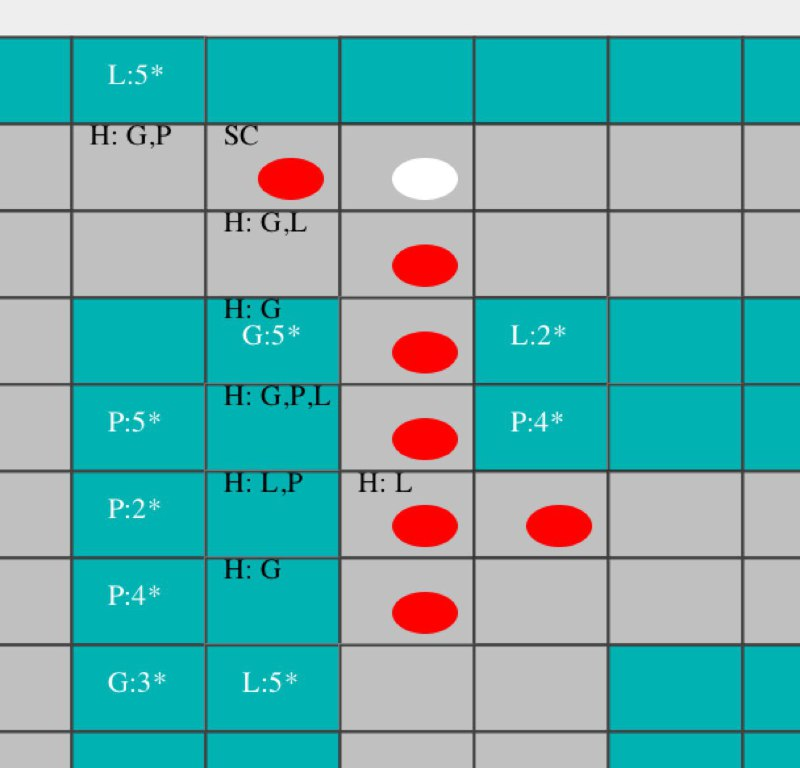
\includegraphics[width=0.5\textwidth]{deadlock}
	\label{deadlock}
	\caption{A typical deadlock in a difficult map topology}
\end{figure}


\section{Tests}

Before arriving at the previously presented conclusions about our implementation's shortcomings, we had run tests on two different maps, comparing two different heuristics for HarvesterAgents: 

\begin{enumerate}
	\item Recycle garbage in closest recycling center (closest)
	\item Maximize benefits per step (best)
\end{enumerate}

\subsection{Jordi's Map}

\begin{figure}[!hbt]
	\centering
	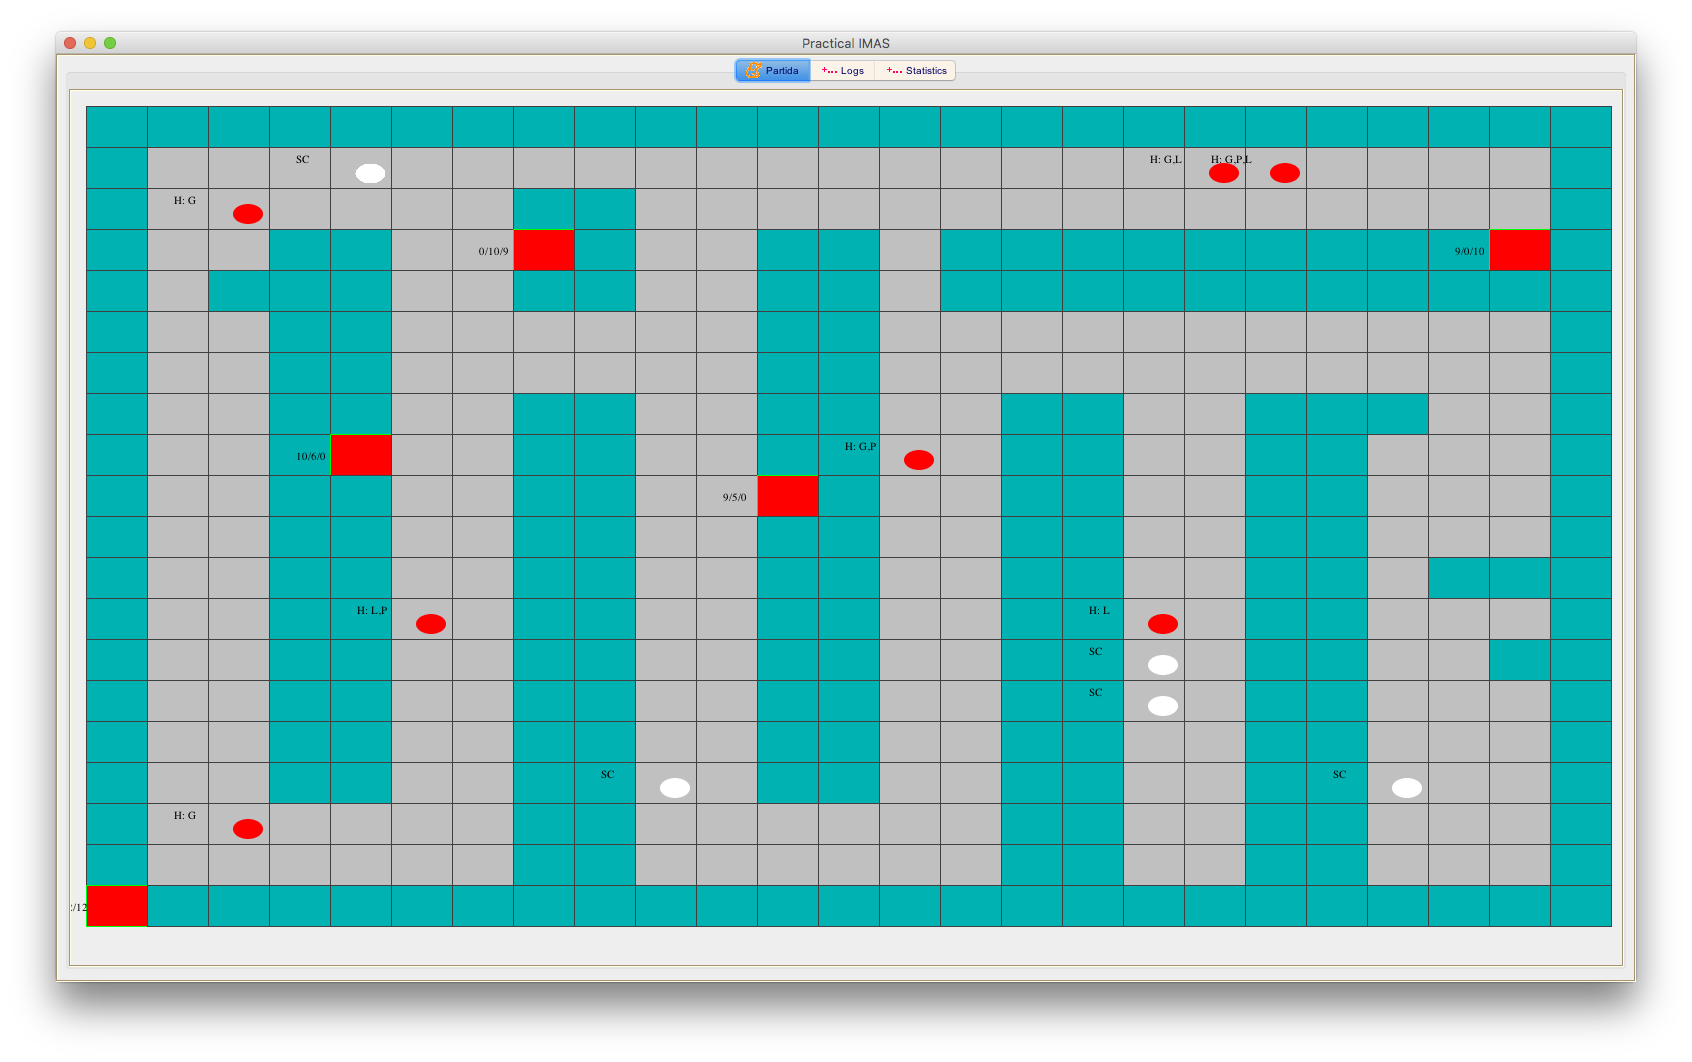
\includegraphics[width=\textwidth]{map_jordi}
	\caption{Jordi's map}
\end{figure}

\begin{table}[!hbt]
	\centering
    \begin{tabular}{ l | r | r }
        \hline
        \textbf{TOTALS} & closest & best \\
		\hline
        Benefits & 2113 & 2454 \\
        G generated & 491 & 508 \\
        G discovered & 460 & 492 \\
        G collected & 254 & 257 \\
        \hline \hline
        \textbf{AVERAGE} & closest & best \\
		\hline
        Benefits/Step & 3.52 & 4.09 \\
        Steps until discovery & 40.72 & 35.70 \\
        Steps until harvesting & 115.04 & 92.69 \\
        \hline \hline
        \textbf{RATIOS} & closest & best \\
		\hline
        G discovered & 0.869 & 0.936 \\
        G collected & 0.517 & 0.506 \\
    \end{tabular}
    \caption{Comparison of results on Jordi's map}
    \label{tab:jordi}
\end{table}

\clearpage

\subsection{Custom Map}

\begin{figure}[!hbt]
	\centering
	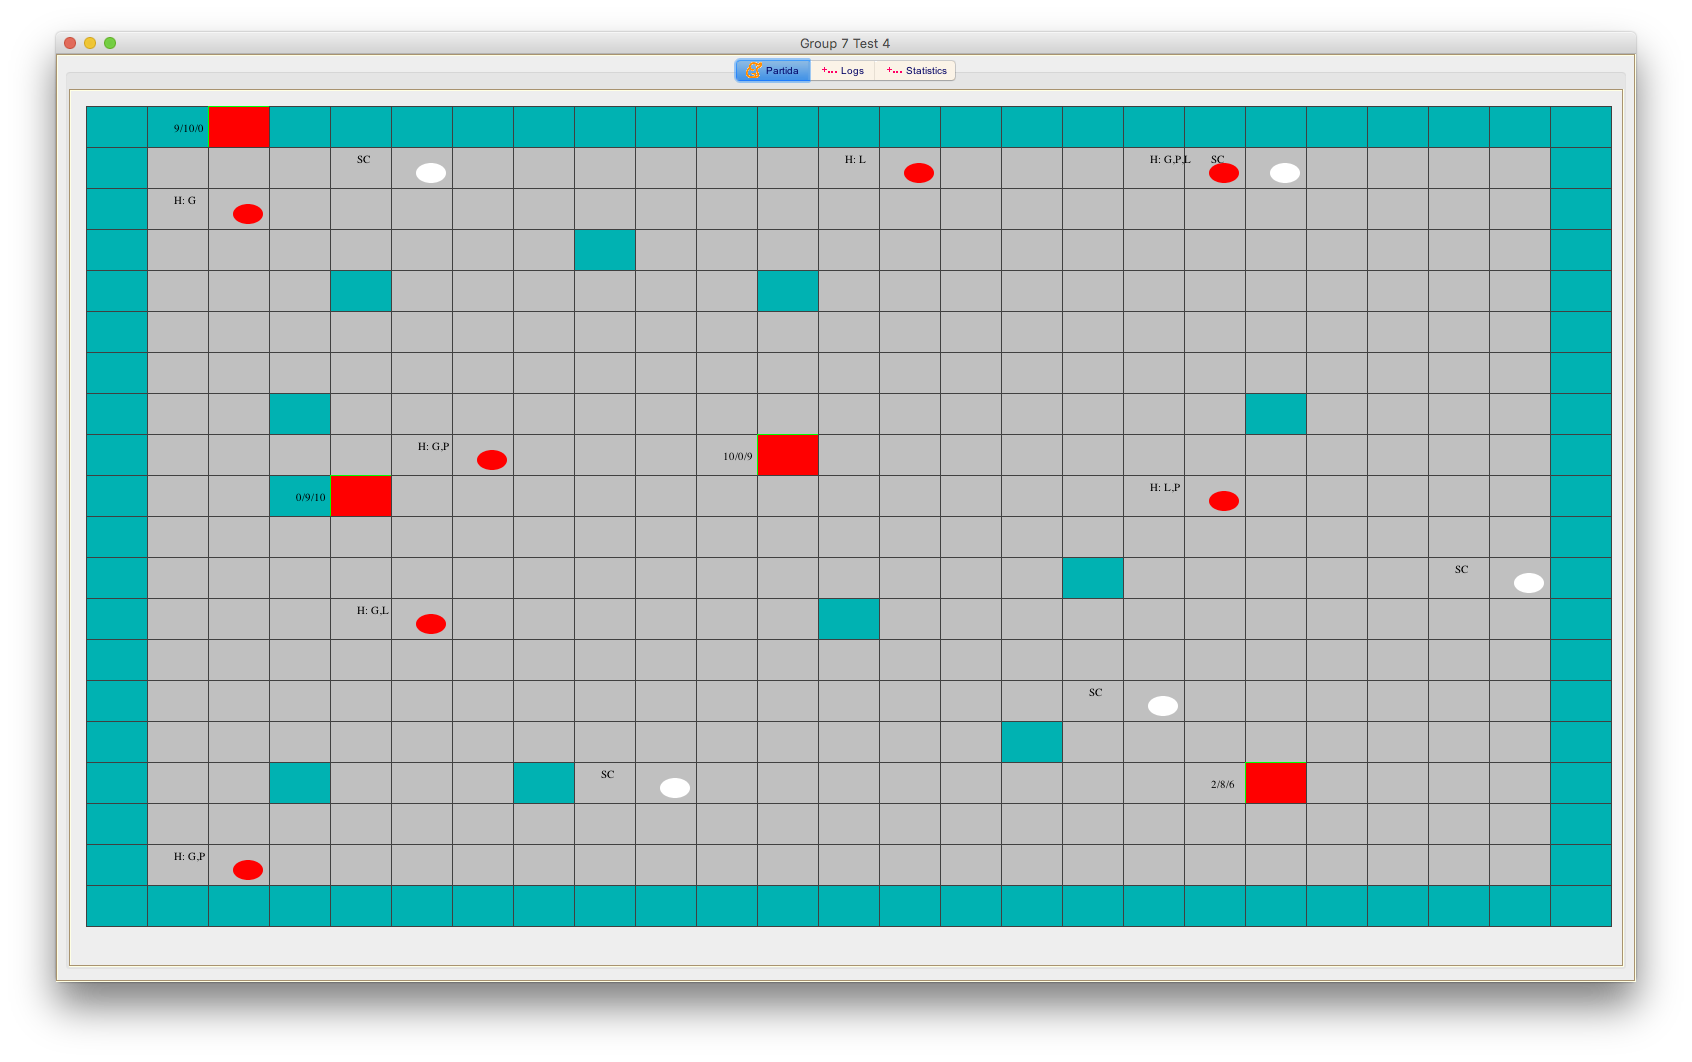
\includegraphics[width=\textwidth]{map_custom}
	\caption{Custom map}
\end{figure}

\begin{table}[!hbt]
	\centering
    \begin{tabular}{ l | r | r }
        \hline
        \textbf{TOTALS} & closest & best \\
		\hline
        Benefits & 3265 & 3755 \\
        G generated & 577 & 555 \\
        G discovered & 569 & 539 \\
        G collected & 415 & 427 \\
        \hline \hline
        \textbf{AVERAGE} & closest & best \\
		\hline
        Benefits/Step & 5.44 & 6.26 \\
        Steps until discovery & 16.95 & 16.94 \\
        Steps until harvesting & 84.31 & 46.06 \\
        \hline \hline
        \textbf{RATIOS} & closest & best \\
		\hline
        G discovered & 0.950 & 0.875 \\
        G collected & 0.719 & 0.769 \\
    \end{tabular}
    \caption{Comparison of results on custom map}
    \label{tab:custom}
\end{table}


